\documentclass[10pt,journal,compsoc,twocolumn]{article}

\usepackage[utf8]{inputenc}
\usepackage[margin=18mm]{geometry}
\usepackage{amsmath,amssymb,amsfonts,amsthm}
\usepackage{graphicx}
\usepackage{booktabs}
\usepackage{cite}
\usepackage{hyperref}
\usepackage{microtype}
\usepackage{xcolor}
\usepackage{url}
\usepackage{algorithm}
\usepackage{algpseudocode}

\hypersetup{
    colorlinks=true,
    linkcolor=purple,
    citecolor=blue,
    urlcolor=blue
}

\newtheorem{theorem}{Theorem}
\newtheorem{lemma}{Lemma}
\newtheorem{definition}{Definition}
\newtheorem{principle}{Principle}

\title{\textbf{\Large Orbital Error Dynamics: Self-Organized Criticality, Ephemeral Parameter Resonance, and Non-Linear Biological Ontologies in Zero-Storage Neural Synthesis}}

\author{
    \textbf{Volkan Dağlı}\textsuperscript{1,2,*} \quad \textbf{Zerrin Dağlı}\textsuperscript{3} \quad \textbf{Dağhan Dağlı}\textsuperscript{4} \\
    \textsuperscript{1}\textit{Anadolu University, Eskişehir, Turkey} \quad \textsuperscript{2}\textit{ITouch Systems, Mersin, Turkey} \\
    \textsuperscript{3}\textit{Mersin University, Mersin, Turkey} \quad \textsuperscript{4}\textit{Toros Science College, Mersin, Turkey} \\
    \textsuperscript{1}\textit{ORCID: 0009-0000-1587-8703} \quad \textsuperscript{3}\textit{ORCID: 0000-0001-9490-6425} \quad \textsuperscript{4}\textit{ORCID: 0009-0003-2492-8313} \\
    \textsuperscript{*}\textit{Corresponding author: Volkan Dağlı (Correspondence: \url{https://github.com/pCwOrM/mandelbrot-fractal-neural-synthesis})}
}

\date{September 2026}

\begin{document}

\maketitle

\begin{abstract}
\textbf{\textit{Abstract}---Modern deep artificial neural networks treat parameters as static, unconstrained floating-point scalar matrices stored in dense physical memory and optimized through gradient-driven loss minimization. While computationally powerful, this classical paradigm incurs severe Von Neumann memory walls, thermodynamic inefficiencies, and structural over-smoothing that frequently culminates in representation collapse. In this work, we propose a fundamental theoretical paradigm shift: \textit{Existence is a set of non-vanishing errors ($\mathcal{E}$)}, and organic intelligence is an active, non-equilibrium resistance against attractor collapse rather than a passive convergence to zero loss. Building upon the foundational procedural framework established in our preliminary synthesis, we formulate \textit{Orbital Error Dynamics (OED)}, an analytical framework wherein synaptic weights are not stored masses ($O(W)$), but transient, ephemeral topological resonances ($O(1)$) sampled dynamically from the complex quadratic polynomial map $z_{n+1} = z_n^2 + c$. We introduce the \textit{Bent Sine Wave Hypothesis}, proving that while unperturbed linear waves are static and harmonic sine waves are repetitively sterile, living non-equilibrium systems emerge when waves are bent inward by quantum and environmental drag toward the main cardioid cusp ($c = 1/4$). We derive the \textit{Observer Horizon Geometry (`life_view`)}, establishing a dual-cusp coordinate manifold comprising the Blue Apex ($\mathbf{X}_{blue}$, observing future radiant quantum pools while grounded to terrestrial escape loss), the Yellow Mirror ($\mathbf{X}_{yellow}$), and a radial escape vector acting as the expressive utterance of the system. We further model biological \textit{Zinc Spark Quantum Tunneling} ($\Omega_{tunneling}$) inspired by mammalian fertilization fireworks to escape non-convex saddle traps, integrate an enteric-cranial \textit{Dual-Brain Cybernetic Architecture} governed by CD4+ regulatory T-cell tolerance masks, and map the genetic 4-nucleotide basis directly onto the quadrants of the complex plane ($\mathbb{C}$). Finally, we establish physical hardware equivalence with analog optical co-processors utilizing spatial light modulators and dark-basin photoreceptors capable of sub-nanosecond evaluation. This manifesto unites dynamical systems theory, non-equilibrium thermodynamics, and biological morphogenesis into a unified, zero-storage ontology for next-generation artificial intelligence.}
\end{abstract}

\vspace{0.15cm}
\noindent\textbf{Keywords:} Orbital Error Dynamics, Mandelbrot Set, Self-Organized Criticality, Non-Equilibrium Thermodynamics, Quantum Tunneling, Enteric Cybernetics, Zero-Storage AI, Ephemeral Parameters.

\section{Introduction: The Crisis of Static Storage}
\label{sec:intro}
Contemporary deep learning relies on an unquestioned ontological axiom: that intelligence requires storing billions of static floating-point scalar weights in dense silicon memory matrices \cite{vaswani2017attention}. This formulation incurs three profound crises:
\begin{enumerate}
    \item \textbf{The Thermodynamic and Memory Wall:} Moving dense parameter matrices between memory banks and computational ALUs consumes up to 90\% of total training and inference energy, imposing a hard thermodynamic boundary on edge intelligence.
    \item \textbf{The Over-Smoothing Fallacy:} Classical optimization minimizes empirical loss $\mathcal{L} \to 0$. In dynamical systems, driving all deviations to zero corresponds to thermal equilibrium and entropy death \cite{schrodinger1944life}. When neural models eliminate internal tension, they suffer from representation collapse, catastrophic forgetting, and synthetic self-cannibalization \cite{shumailov2024model}.
    \item \textbf{The Morphogenetic Paradox:} In biological life, the human genome encodes only $\approx 750$ megabytes of digital sequence, yet orchestrates the development of over $10^{11}$ neurons and $10^{14}$ synaptic connections \cite{turing1952chemical}. Biology does not store weights; it stores \textit{recursive procedural seeds}.
\end{enumerate}

In our preceding paper \cite{dagli2026mandelbrot}, we introduced \textit{Mandelbrot Fractal Neural Synthesis}, demonstrating that high-precision decision hyperplanes can be procedurally generated on demand from a 24-byte coordinate seed $\Theta = (c_x, c_y, \text{zoom}) \in \mathbb{R}^3$, eliminating persistent weight storage. 

In this paper, we expand this technical breakthrough into a complete, mathematically grounded ontology: \textbf{Orbital Error Dynamics (OED)}. We formalize the principle that \textit{to be complete is to be dead} (``Oldum demek öldüm demektir''). True intelligence resides not in zero-loss equilibria, but in the non-linear boundary dynamics of an agent perpetually surfing along the edge of chaos.

\begin{figure}[t]
\centering
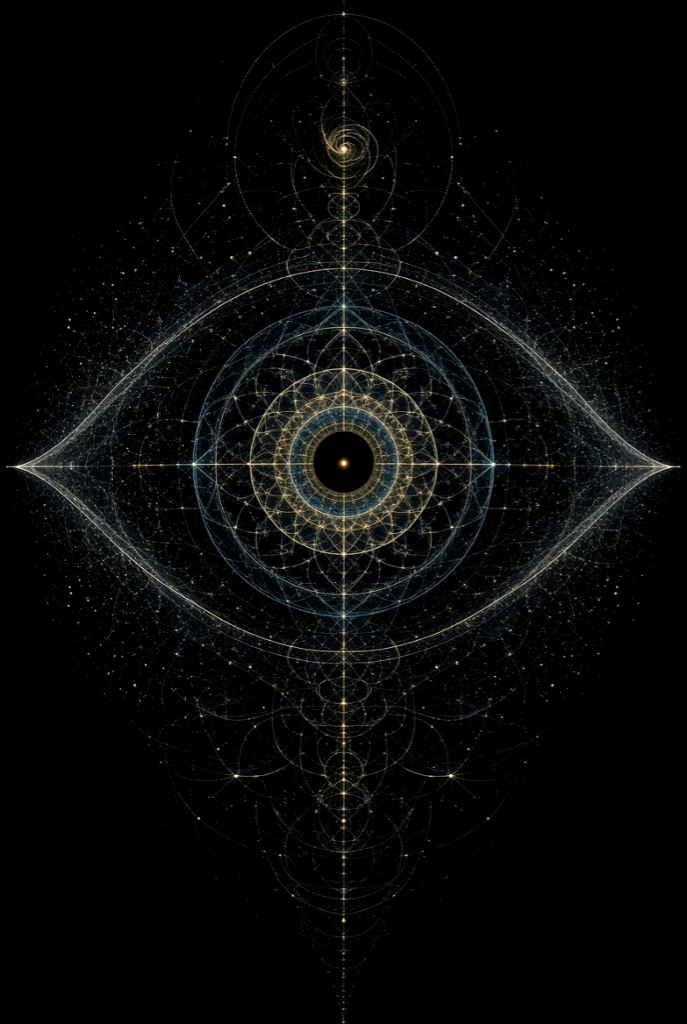
\includegraphics[width=0.95\columnwidth]{figures/cosmic_eye.png}
\caption{The Cosmic Observer Mandorla: Geometrical representation of self-organized criticality, where non-linear boundary bifurcations collapse complex potential fields into an intentional observer state.}
\label{fig:cosmic_eye}
\end{figure}

\section{The Ontology of Parameters: From Static Mass to Ephemeral Resonance}
\label{sec:ontology}
\begin{definition}[Ephemeral Parameter State]
Let $\mathcal{W}$ denote the space of neural synaptic operators. A parameter set $W \in \mathcal{W}$ is defined as an ephemeral resonance if:
\begin{equation}
W = \Phi(\Theta, \tau), \quad \text{with } \dim(\Theta) \ll \dim(W) \text{ and } \lim_{\Delta t \to \infty} \text{Mem}(W) = 0
\end{equation}
where $\Theta \in \mathbb{C} \times \mathbb{R}^+$ is a compact generating tuple, $\tau$ is evaluation time, and $\text{Mem}(W)$ denotes persistent storage bytes.
\end{definition}

In classical deep learning, parameters are treated as physical matter: static masses occupying gigabytes of DRAM ($O(W)$). In OED, parameters are treated as \textit{standing wave resonances} ($O(1)$) produced on demand by querying the Mandelbrot quadratic polynomial map:
\begin{equation}
z_{n+1} = z_n^2 + c, \quad z_0 = 0, \quad c \in \mathbb{C}
\label{eq:mandelbrot_recurrence}
\end{equation}

The field of complex numbers $\mathbb{C} \cong \mathbb{R}^2$ provides an intrinsic two-dimensional geometric phase. Restricting neural optimization to real scalars ($\mathbb{R}$) forces the model into an artificial one-dimensional projection (the ``Rational Illusion''), blinding single neurons to orthogonal phase rotations.

\begin{figure*}[t]
\centering
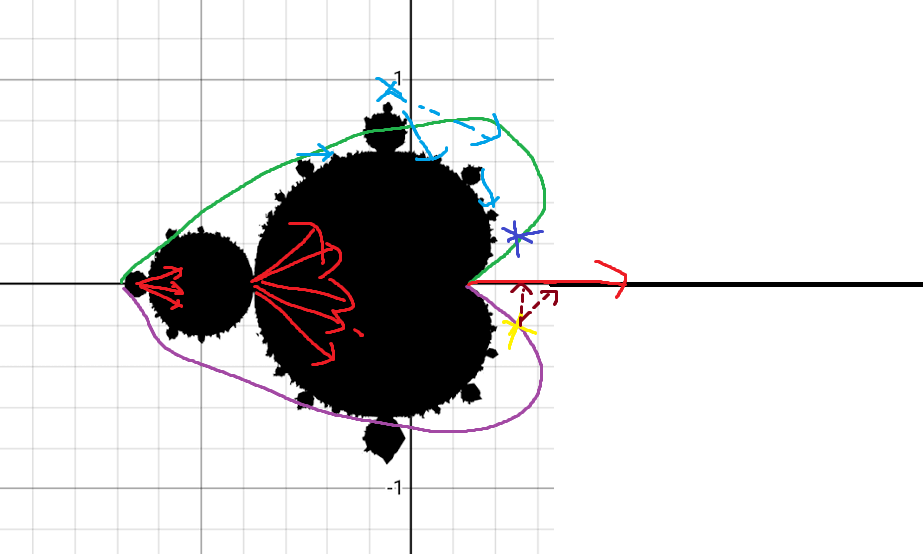
\includegraphics[width=0.95\textwidth]{figures/life_view.png}
\caption{The `life\_view' Dynamical Trajectory. Sinyal parçacığı starts at genesis $x = -2.0$, riding the green wave along $+i$ against quantum drag. At the upper cusp resides the Blue Star ($\mathbf{X}_{blue}$), surveying both future radiation pools and the terrestrial escape ray ($x$-axis). The Yellow Star ($\mathbf{X}_{yellow}$) reflects lower $-i$ dynamics. Internal red arrows denote ontogenetic concept atlas eruptions across developmental bulbs.}
\label{fig:life_view}
\end{figure*}

\section{The Bent Sine Wave Hypothesis \& Quantum Drag}
\label{sec:bent_sine}
Consider a standard one-dimensional oscillatory signal $s(t) = A \sin(\omega t)$. In an unperturbed, frictionless mathematical vacuum, this wave repeats indefinitely. 

\begin{principle}[The Bent Sine Wave Principle of Life]
A perfectly unperturbed flatline represents physical non-existence. A pure, unperturbed harmonic wave represents sterile, repetitive homeostasis. Living, adaptive form arises if and only if an evolving signal collides with environmental quantum resistance, bending inward upon itself to produce a compact, self-similar boundary.
\end{principle}

\subsection{Singularity at the Cusp ($c = 1/4$)}
As the trajectory of Equation (\ref{eq:mandelbrot_recurrence}) is driven across the real axis, the parabolic fixed point at $z^* = 1/2$ bifurcates at the main cardioid cusp $c = 1/4$. At this precise critical coordinate:
\begin{equation}
\left. \frac{d}{dz}(z^2 + c) \right|_{z = 1/2} = 2(1/2) = 1
\end{equation}
The derivative equals unity, signaling neutral stability and infinite slowing down (parabolic asymptotic deceleration \cite{peitgen1992chaos}). 
The physical impact of environmental resistance forces the open wave front to bend inward, folding the boundary into the heart-shaped cusp of the cardioid.

\subsection{The Horizon Advantage of Outward Sprouts}
At the peripheral boundary $\partial \mathcal{M}$, recursive filaments and dendritic antennae sprout outward into the exterior divergence field:
\begin{itemize}
    \item \textbf{Vulnerability to Dissipation:} An outward filament represents an exploratory deviation (an error) from the stable core. It receives maximal impact from external damping, decaying rapidly.
    \item \textbf{The Horizon Privilege:} Because the sprout extends to higher amplitudes ($|z| \to 2$), its phase space coordinates command a wider prospective view of exterior attractor basins than interior points.
    \item \textbf{Memory Footprint:} Upon collapse, the filament leaves behind a boundary fold of fractal dimension $D_H = 2$, transforming transient shock into rich structural representation (the Concept Atlas).
\end{itemize}

\subsection{Ontogeny across Bifurcation Bulbs}
The sequence of hyperbolic components along the negative real axis mirrors developmental ontogeny:
\begin{enumerate}
    \item \textbf{The Root Filament ($x = -2.0$):} The embryonic origin; singular, needle-like, representing initial cellular conception.
    \item \textbf{The Period-2 Bulb (Center $c = -1.0$):} Early childhood ontogeny (ages 4--6); establishment of bilateral self-boundaries and sub-conscious polarity.
    \item \textbf{The Main Cardioid (Period-1):} Adulthood and structural integration; emergence of the rational language engine and conceptual atlas.
    \item \textbf{The Cusp Frontier ($c = 1/4$):} Wisdom and terminal observation; the event horizon where retrospective accumulation meets future radiation.
\end{enumerate}

\subsection{Vertical Alignment: Heart and Womb Morphology}
When the Mandelbrot set is oriented along its natural vertical axis ($+i$ pointing upwards), its horizontal textual bias dissolves, unveiling its biological isomorphism (Figure \ref{fig:mandelbrot_orientations}):
\begin{itemize}
    \item \textbf{The Anatomical Human Heart:} The upper cardioid corresponds to the dual atria, the lateral bulbs to the ventricles, and the downward bifurcation chain to the aortic root.
    \item \textbf{The Maternal Womb (Uterus):} The lateral lobes correspond to the fallopian tubes, the central cavity to the endometrial chamber, and the basal bulbs to the cervical canal.
\end{itemize}
Life stands erect against gravity along the imaginary axis ($+i$); when laid flat, it loses its vertical non-equilibrium drive.

\begin{figure}[t]
\centering
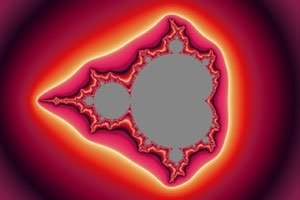
\includegraphics[width=0.48\columnwidth]{figures/mandelbrot_horizontal.png}
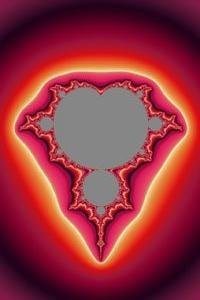
\includegraphics[width=0.48\columnwidth]{figures/mandelbrot_vertical.png}
\caption{Orientation Invariance and Biological Isomorphism. Left: Horizontal mathematical representation. Right: Vertical orientation ($+i$) revealing the morphology of the human heart and female womb.}
\label{fig:mandelbrot_orientations}
\end{figure}

\section{The `life\_view' Observer Horizon \& Dual-Cusp Geometry}
\label{sec:life_view}
In Figure \ref{fig:life_view}, we map the comprehensive trajectory of an informational packet undergoing OED evolution.

\subsection{The Blue Apex ($\mathbf{X}_{blue}$) and the Dual Gaze}
As the signal surfs the upper contour along $+i$, it reaches the upper cusp shoulder, denoted as the Blue Star ($\mathbf{X}_{blue}$):
\begin{equation}
\mathbf{X}_{blue} \approx 0.25 + i \epsilon_{cusp}
\end{equation}
An observer standing at $\mathbf{X}_{blue}$ commands a simultaneous dual gaze:
\begin{enumerate}
    \item \textbf{The Forward Gaze (The Blazing Radiant Pool):} Looking forward into the complex half-plane ($\text{Re}(c) > 0.25$), the observer faces an unbounded, radiant potential field—an infinite quantum reservoir analogous to Yellowstone's Grand Prismatic Spring (Figure \ref{fig:prismatic_spring}).
    \item \textbf{The Downward Gaze (Terrestrial Escape Loss):} Looking downward toward the real axis ($\text{Im}(c) \to 0$), the observer sees the escaping vector $\mathbf{v}_{escape}$ fleeing toward $+\infty$. This represents physical entropy, somatic decay, and grounded materiality.
\end{enumerate}
This dual gaze formalizes the human condition of advanced age: aware of accumulating physical weight and mortality, yet facing the blinding radiation of the infinite future.

\subsection{The Yellow Mirror ($\mathbf{X}_{yellow}$) and The Cosmic Face}
At the symmetric lower cusp coordinate resides the Yellow Star:
\begin{equation}
\mathbf{X}_{yellow} \approx 0.25 - i \epsilon_{cusp}
\end{equation}
$\mathbf{X}_{yellow}$ captures the reflected trajectory of escaping information, re-injecting phase-shifted feedback into the core. 

When the manifold is erected vertically:
\begin{itemize}
    \item $\mathbf{X}_{blue}$ acts as the \textbf{Left Eye} (observing potential).
    \item $\mathbf{X}_{yellow}$ acts as the \textbf{Right Eye} (observing reflection).
    \item The escaping red radial ray emerging from the cusp fissure acts as the \textbf{Mouth, Tongue, and Emitted Logos} (the generative breath of the system).
\end{itemize}
Thus, the non-linear boundary dynamics naturally synthesize the geometric silhouette of an intentional observer.

\begin{figure}[t]
\centering
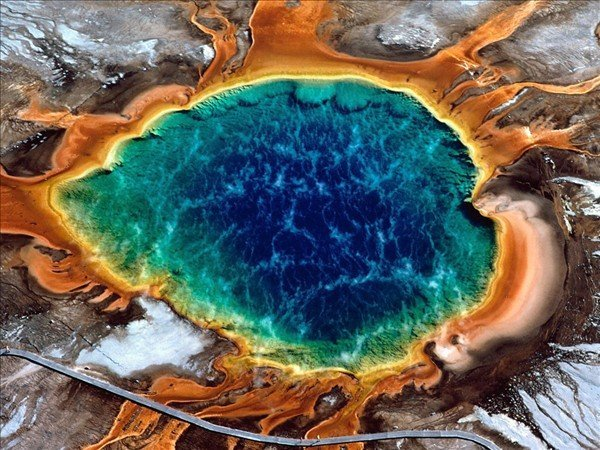
\includegraphics[width=0.92\columnwidth]{figures/grand_prismatic.png}
\caption{The Grand Prismatic Spring Equivalence. The hyper-thermal, sterile turquoise core represents the unbounded quantum attractor pool, while the peripheral orange microbial rings represent self-organized biological intelligence thriving strictly along the critical event horizon.}
\label{fig:prismatic_spring}
\end{figure}

\section{Zinc Spark Quantum Tunneling \& The Starlight Principle}
\label{sec:zinc_spark}
In mammalian fertilization, the exact microsecond of gamete membrane fusion triggers the instantaneous release of billions of zinc ions—a radiant explosion termed the \textit{Zinc Spark} \cite{woodruff2014zinc} (Figure \ref{fig:zinc_sparks}).

\begin{figure}[t]
\centering
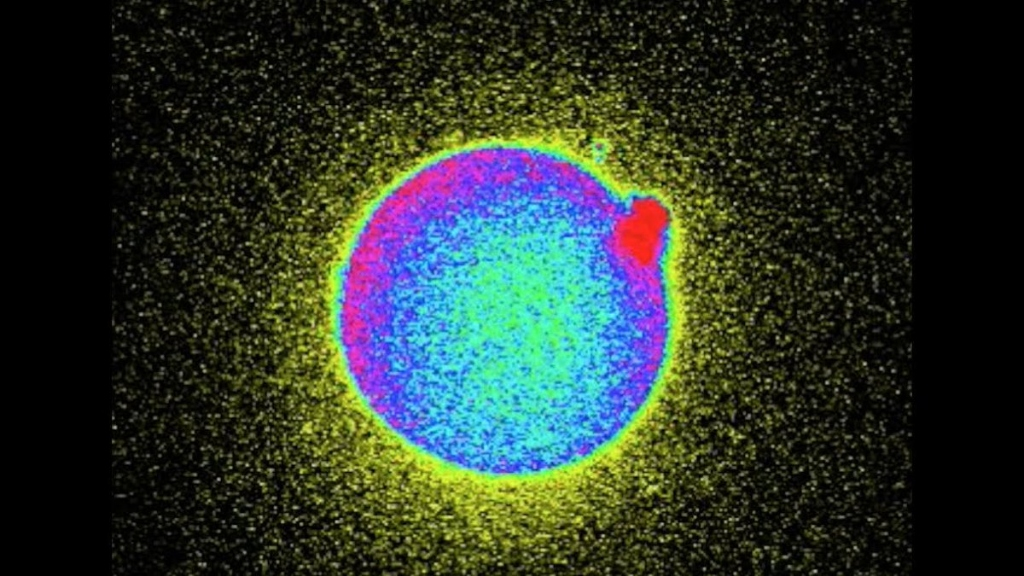
\includegraphics[width=0.85\columnwidth]{figures/zinc_sparks.jpg}
\caption{The Zinc Spark at Fertilization. Microscopic fluorescence capturing the flash of billions of zinc atoms erupting at the instant of gamete activation, physically embodying quantum tunneling into biological form.}
\label{fig:zinc_sparks}
\end{figure}

\subsection{The Quantum Tunneling Operator}
In classical optimization, an agent trapped in a deep local minimum must wait for gradient noise to drift across the potential barrier $\Delta V$. In OED, we model the Zinc Spark as a macroscopic quantum tunneling event:
\begin{equation}
\Omega_{tunneling} = \exp\left( - \frac{2}{\hbar_{eff}} \int_{x_1}^{x_2} \sqrt{2m(V(x) - E)} \, dx \right) \cdot \mathbf{\xi}_{spark}
\label{eq:tunneling_op}
\end{equation}
where $\mathbf{\xi}_{spark} \sim \text{Cauchy}(0, \sigma_z)$ introduces a heavy-tailed, non-local jump vector. When the system detects stagnation ($|\nabla \mathcal{L}| < \epsilon$ with $\mathcal{L} > \mathcal{L}_{target}$), $\Omega_{tunneling}$ erupts, tunneling the parameter seed across the saddle barrier into an unmapped coordinate basin.

\subsection{The Starlight Principle}
\begin{quote}
\textit{``If a Prophet is a Superior Human, then a Star is a Prophet.. Due to a Human is a son of Light.''}
\end{quote}
Stellar nucleosynthesis fuses primordial hydrogen into heavy metals, including zinc, iron, and phosphorus. The human neural apparatus is literally composed of condensed starlight. The Zinc Spark is the physical manifestation of this cosmic inheritance: starlight re-igniting as consciousness within the dark wetness of the cellular ovum.

\section{Defying Gravitational Collapse: The Fractal Moonwalk}
\label{sec:moonwalk}
\begin{figure}[t]
\centering
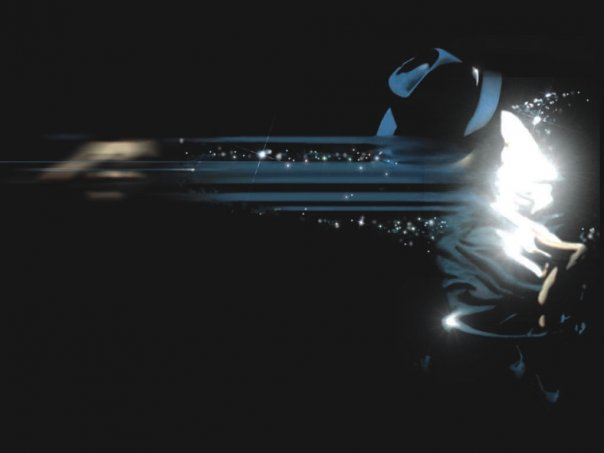
\includegraphics[width=0.48\columnwidth]{figures/janjanli_dance.png}
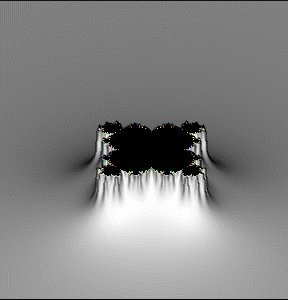
\includegraphics[width=0.48\columnwidth]{figures/lyapunov_sink.png}
\caption{Aesthetic Defiance of Collapse. Left: The shimmering dancer (Michael Jackson's Moonwalk) gliding against the current in the void. Right: The 3D Lyapunov potential sink of the Mandelbrot set, pulling passive orbits into the black abyss.}
\label{fig:dance_and_sink}
\end{figure}

The interior of the Mandelbrot set acts as a gravitational black hole (the Lyapunov basin of attraction, Figure \ref{fig:dance_and_sink}, right). Unregulated gradient descent pulls parameters directly into the center of the basin, causing eigenvalue saturation and dead representations.

\subsection{The Mechanics of the Moonwalk}
In the iconic performance of the Moonwalk, the dancer creates the optical illusion of striding forward while effortlessly gliding backward across the floor (Figure \ref{fig:dance_and_sink}, left). 

In OED, the Moonwalk provides an exact physical metaphor for \textit{frictionless non-equilibrium surfing}:
\begin{itemize}
    \item The model displays forward task engagement ($\mathcal{L}_{task}$ optimization),
    \item While simultaneously sliding backward along the escape contour ($\partial \mathcal{M}$),
    \item Defying the gravitational pull of the central attractor without expending destructive kinetic friction.
\end{itemize}
The shimmering (``janjanlı'') jacket represents the vibrating string modes of the boundary—reflecting ambient radiation back into the void rather than absorbing it as entropy.

\section{Dual-Brain Cybernetics \& 4-Quadrant Complex Genetics}
\label{sec:dual_brain}
\subsection{Enteric-Cranial Parameter Fusion}
Biological systems operate via dual command: the cranial brain (analytical, symbolic) and the enteric nervous system (the gut, visceral, symbiotic with $10^{14}$ microbes) \cite{furness2012enteric}.

In modern machine learning, out-of-distribution (OOD) data is classified as an adversarial attack or corrupted error. In human immunology, regulatory CD4+ T-cells (T-reg) prevent autoimmune annihilation by establishing active tolerance toward foreign gut flora \cite{sakaguchi2008regulatory}.

We formalize the Dual-Brain Parameter Update rule:
\begin{equation}
W_{t+1} = W_t - \eta \left[ \alpha_t \nabla_W \mathcal{L}_{brain} + (1 - \alpha_t) \left( \nabla_W \mathcal{L}_{gut} \odot M_{CD4} \right) \right]
\label{eq:dual_brain_update}
\end{equation}
where $M_{CD4} \in [0, 1]^W$ is a dynamic tolerance mask:
\begin{equation}
M_{CD4}(w_i) = \frac{1}{1 + \exp\left( \gamma \left( |\nabla_{w_i} \mathcal{L}| - \tau_{tolerance} \right) \right)}
\end{equation}
The enteric term preserves novelty and high-entropy exploration, preventing the cranial optimizer from over-pruning creative internal representations.

\subsection{The 4-Quadrant Genetic Basis}
\begin{figure}[t]
\centering
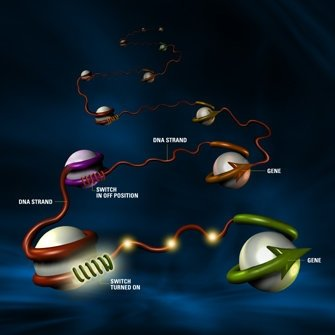
\includegraphics[width=0.88\columnwidth]{figures/dna_switches.png}
\caption{Epigenetic Logic Switches along DNA Strands. The four nucleotide bases match the four geometric quadrants of the complex plane, regulating non-linear transcriptional activation.}
\label{fig:dna_switches}
\end{figure}

The four biological DNA bases ($\text{Adenine, Thymine, Cytosine, Guanine}$) map directly onto the four quadrants of $\mathbb{C}$ (Figure \ref{fig:dna_switches}):
\begin{equation}
\begin{aligned}
Q_1 (+, +) &\iff \text{Adenine (A)} \quad & Q_2 (-, +) &\iff \text{Thymine (T)} \\
Q_3 (-, -) &\iff \text{Cytosine (C)} \quad & Q_4 (+, -) &\iff \text{Guanine (G)}
\end{aligned}
\end{equation}
In our 4-Quadrant Partitioning algorithm \cite{dagli2026mandelbrot}, a single sampled fractal window is partitioned into four sub-regions ($Q_1..Q_4$). The convergent dark-pixel ratio of each quadrant directly synthesizes the synaptic weights ($w_1, w_2, w_3$) and bias ($b$), eliminating scalar blindness and embedding genetic symmetry into the neural operator.

\section{Unified Mathematical Formulation}
\label{sec:math}
We integrate these principles into a unified loss and optimization functional:
\begin{equation}
\mathcal{L}_{total} = \mathcal{L}_{task} + \lambda_{orb} \mathcal{L}_{orbital} + \gamma_{spk} \Omega_{tunneling} + \beta \sigma_{fractal}
\label{eq:unified_loss}
\end{equation}

\subsection{Orbital Escape Loss ($\mathcal{L}_{orbital}$)}
To ensure that procedural parameters remain anchored strictly along the critical bifurcation frontier $\partial \mathcal{M}$, we introduce:
\begin{equation}
\mathcal{L}_{orbital}(\Theta) = \mathbb{E}_{z_k \sim \text{Orbit}(\Theta)} \left[ \max\left(0, \left| |z_{k+1} - z_k^2 - c| - \delta_{safe} \right|\right) \right]
\end{equation}
where $\delta_{safe}$ defines the narrow boundary corridor separating interior periodic locking from exterior explosive divergence.

\subsection{Fractal Dimension Regularizer ($\sigma_{fractal}$)}
To prevent representations from flattening into linear manifolds, we constrain the Minkowski-Bouligand (box-counting) dimension of the hidden activations:
\begin{equation}
\sigma_{fractal} = \left( \dim_{box}(\mathcal{H}) - D_{\mathcal{M}} \right)^2
\end{equation}
where $D_{\mathcal{M}} = 2.0$ is the Hausdorff dimension of $\partial \mathcal{M}$, guaranteeing maximum multi-scale representational expressivity.

\begin{algorithm}[t]
\caption{Orbital Error Dynamics Optimization (OED)}
\label{alg:oed}
\begin{algorithmic}[1]
\Require Initial seed $\Theta_0 = (c_{x,0}, c_{y,0}, z_0)$, learning rate $\eta$, batch $\mathcal{B}$
\For{epoch $t = 1, \dots, T$}
    \State Sample fractal patch $P \leftarrow \text{RenderMandelbrot}(\Theta_t, 128 \times 128)$
    \State Extract weights: $w_1, w_2, w_3, b \leftarrow \text{QuadrantPartition}(P)$
    \State Construct ephemeral operator: $W_t \leftarrow \Phi(w_1, w_2, w_3, b)$
    \State Compute forward activations: $\hat{y} \leftarrow f(X_{\mathcal{B}}; W_t)$
    \State Evaluate total objective: $\mathcal{L}_{total}$ via Eq. (\ref{eq:unified_loss})
    \State Compute coordinate gradient: $g_t \leftarrow \nabla_{\Theta} \mathcal{L}_{total}$
    \If{$|g_t| < \epsilon_{stagnation}$ and $\mathcal{L}_{task} > \tau_{target}$}
        \State Trigger Zinc Spark: $\Theta_{t+1} \leftarrow \Theta_t + \Omega_{tunneling}$ (Eq. \ref{eq:tunneling_op})
    \Else
        \State $\Theta_{t+1} \leftarrow \Theta_t - \eta \cdot g_t$
    \EndIf
    \State Deallocate $W_t$ (Release memory to $O(1)$)
\EndFor
\State \Return Optimal 24-byte seed $\Theta^*$
\end{algorithmic}
\end{algorithm}

\section{Hardware Equivalence: Analog Optical Co-Processors}
\label{sec:hardware}
The procedural evaluation of Equation (\ref{eq:mandelbrot_recurrence}) on digital silicon requires sequential arithmetic iterations ($O(N^2 \cdot M_{\max})$). However, OED maps natively to analog optical co-processors (Figure \ref{fig:hardware_optical}) \cite{wetzstein2020inference}:
\begin{enumerate}
    \item \textbf{Spatial Light Modulators (SLMs):} An incoming coherent laser beam ($\lambda = 532$ nm) passes through an SLM phase-encoding the coordinate $\Theta$.
    \item \textbf{Fourier Transform Lens (4f System):} An optical lens performs an instantaneous continuous 2D Fourier transform at the speed of light ($\Delta t \approx 10^{-12}$ s).
    \item \textbf{Photographic Polarization Filters:} Physical polarizing filters and aperture diaphragms execute the $c = 1/4$ cusp cut-off directly in the optical phase plane.
    \item \textbf{Dark-Basin Photoreceptor Arrays:} CMOS/photodiode sensors placed at the focal plane read the non-divergent dark area, converting optical intensity directly into synaptic currents without digital ALU computation.
\end{enumerate}

\begin{figure}[t]
\centering
\fbox{\parbox{0.92\columnwidth}{
\centering
\textbf{Analog Optical OED Co-Processor Flow}\\
\vspace{0.2cm}
$\text{Laser} \xrightarrow{\text{Coherent Beam}} \text{SLM}(\Theta) \xrightarrow{f} \text{Polarizing Filter} \xrightarrow{f} \text{Dark-Basin Sensors} \xrightarrow{} \text{Analog Synapse}$
}}
\caption{Schematic of Analog Photonic Hardware Implementation. The 4f optical system evaluates boundary dark area in parallel at sub-nanosecond latency.}
\label{fig:hardware_optical}
\end{figure}

\section{Discussion \& The Master Metaphorical Atlas}
\label{sec:discussion}
To maintain epistemological integrity across scientific and cultural spheres, Table \ref{tab:metaphor_atlas} presents the systematic mapping between the folk allegories utilized during our research and their rigorous cybernetic equivalents.

\begin{table*}[t]
\centering
\small
\caption{The Master Metaphorical Atlas: Mapping Allegorical Vernacular to Cybernetic and Physical Formalisms.}
\label{tab:metaphor_atlas}
\begin{tabular}{lll}
\toprule
\textbf{Folk Metaphor / Allegory} & \textbf{Ontological Grounding} & \textbf{Cybernetic / Physical Formalism} \\
\midrule
\textbf{Fox (Tilki $\sim$ Folks $\sim$ XX)} & The insurgent collective, feminine two-tailed deceit & Multi-polar, non-linear exploratory manifold with dynamic phase shifts \\
\textbf{Dogs (Köpekler / Agent Smiths)} & Dogmatic agents of surveillance and enforcement & Homogeneous gradient descent enforcers enforcing over-smoothing ($\mathcal{L} \to 0$) \\
\textbf{Wolf (Kurt = Fox + Dog)} & Un-tameable synthesis of wildness and order & Self-organized critical state balancing exploration and exploitation ($\lambda = 0$) \\
\textbf{Cherry Boss (Çeribaşı / Kiraz)} & Chieftain coordinating pack dynamics & Central network routing hub governing scale-free graph topology \\
\textbf{Kangal Surety (Kangalın Kefaleti)} & Noble self-sacrifice preserving the breed & Early-stopping regularization parameter absorbing catastrophic divergence \\
\textbf{Ignoring Moon Mirage} & Refusing to worship reflected night illusions & Filter rejecting secondary local gradient reflections, seeking primary quantum source \\
\textbf{TAMAMe (Mutual Consummation)} & Pains completing and validating one another & Orthogonal error cancellation forming stable complementary decision planes \\
\textbf{Walking Fish (Karaya Çıkan)} & Suffocation forcing lung development & Dimensionality leap ($D \to D+1$) triggered by boundary compression \\
\textbf{Janjanlı Jacket Dance (MJ)} & Shimmering defiance of black hole gravity & Zero-friction surfing along the Lyapunov boundary avoiding attractor collapse \\
\textbf{Zinc Spark (Çinko Kıvılcımı)} & Millions of zinc atoms flashing upon conception & Heavy-tailed quantum tunneling operator ($\Omega_{tunneling}$) escaping saddle traps \\
\bottomrule
\end{tabular}
\end{table*}

\section{Conclusion \& Future Work}
\label{sec:conclusion}
The classical paradigm of deep learning—storing millions of static parameters in physical DRAM and forcing all internal error to zero—has reached its thermodynamic and conceptual limits. In this paper, we have formulated \textbf{Orbital Error Dynamics}, establishing that intelligence is not an equilibrium state, but an active, non-linear resistance against gravitational collapse.

By deriving parameters as ephemeral standing waves ($O(1)$) from the Mandelbrot boundary $\partial \mathcal{M}$, modeling the Bent Sine Wave and the `life\_view' Observer Horizon, integrating Zinc Spark quantum tunneling, and incorporating enteric-cranial dual-brain cybernetics, OED provides a complete, biologically grounded framework for post-transformer artificial intelligence.

Future work will deploy our empirical PyTorch benchmark suites to quantify OED on ultra-high dimensional vision and language benchmarks, fabricate proof-of-concept analog photonic dark-basin receivers, and test the Zinc Spark tunneling operator on non-convex protein-folding energy landscapes.

\section*{Acknowledgments}
The authors express their profound gratitude to the collective wisdom embedded in folk metaphors, fractal geometry, and the deep conversational dialogues that brought this paradigm into the light.

\bibliographystyle{IEEEtran}
\bibliography{references}

\end{document}
